\documentclass{scrartcl}
\usepackage[utf8]{inputenc}
\usepackage{pgfplots}
\pgfplotsset{compat=1.4}
\begin{document}

\begin{figure}
  \centering
  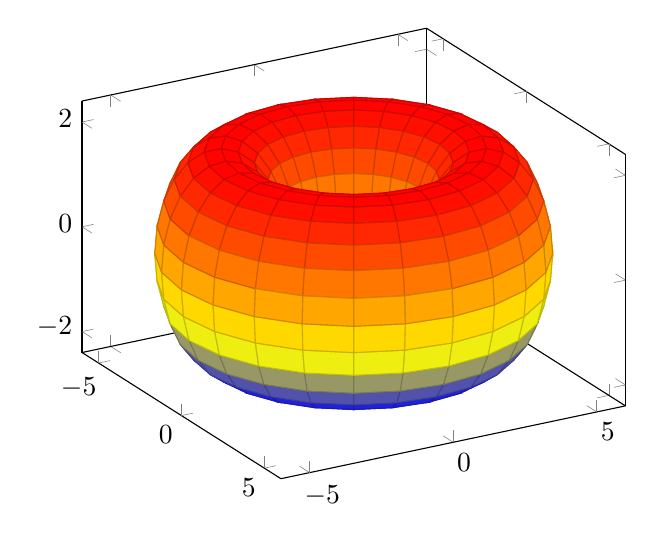
\begin{tikzpicture}
    \newcommand*\radius{2}
    \newcommand*\Radius{4}
    \begin{axis}[view={60}{30}]
      \addplot3[surf, domain=0:2*pi,z buffer=sort]
         ({(\Radius + \radius * cos(deg(y))) * cos(deg(x))},
         {(\Radius + \radius * cos(deg(y))) * sin(deg(x))},
         {\radius * sin(deg(y))});
    \end{axis}
  \end{tikzpicture}
  \caption{Torus}
\end{figure}

\begin{figure}
  \centering
  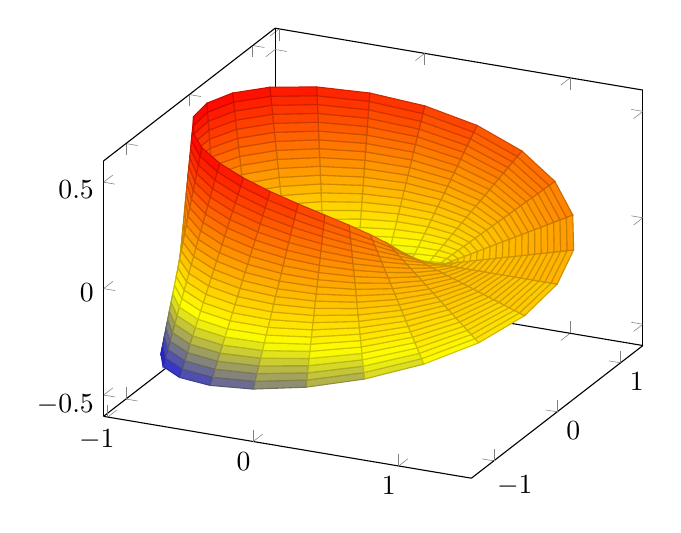
\begin{tikzpicture}
    \begin{axis}
      \addplot3[surf,domain=-1:1,y domain=0:2*pi,z buffer=sort]
         ({cos(deg(y)) * (1 + x/2 * cos(deg(y)/2))},
         {sin(deg(y)) * (1 + x/2 * cos(deg(y)/2))},
         {x/2 * sin(deg(y)/2)});
    \end{axis}
  \end{tikzpicture}
  \caption{M\"obiusband}
\end{figure}

\begin{figure}
  \centering
  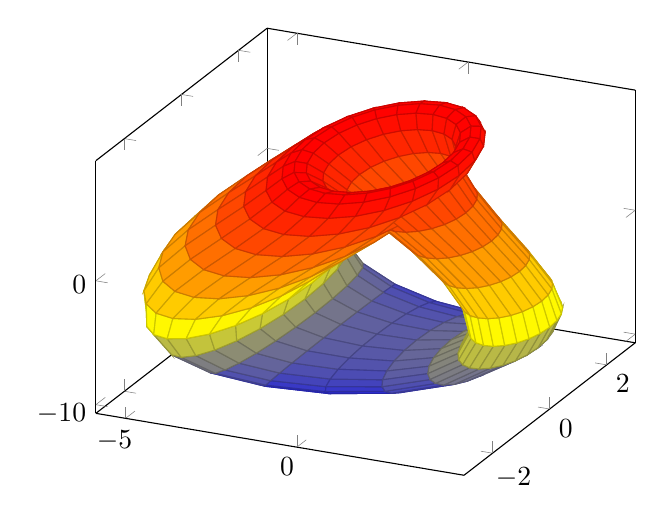
\begin{tikzpicture}
    \newcommand*\breite{3}
    \newcommand*\hoehe{8}
    \begin{axis}
      \addplot3[surf,domain=0:2*pi,z buffer=sort]
         ( { \breite * ( 1 - sin(deg(x))) * cos(deg(x)) + (2 - cos(deg(x))) * cos(deg(y)) * ( 2 * exp(-(x/2 - pi)^2) -1 ) } ,
           { ( 2 - cos(deg(x)) ) * sin(deg(y)) } ,
           { \hoehe * sin(deg(x)) + .5 * ( 2 - cos(deg(x)) ) * sin(deg(x)) * cos(deg(y)) * exp(-(x -3*pi/2)^2) } );
    \end{axis}
  \end{tikzpicture}
  \caption{Klein'sche Flasche}
\end{figure}

\end{document}